\section{Performance} \label{Performance}

This section discusses preliminary performance of the FEC using physics data production runs from Fall 2018.  This run period used beam energies of 10.6, 7.5 and 6.5 GeV with the CLAS12 torus magnet polarity set for both inbending and outbending electrons.  The data presented here used the standard FEC FPGA-based electron trigger with a 15 kHz trigger rate and beam currents of 40 nA on a 5~cm LH$_2$ target.

\begin{figure}[t]
\centering
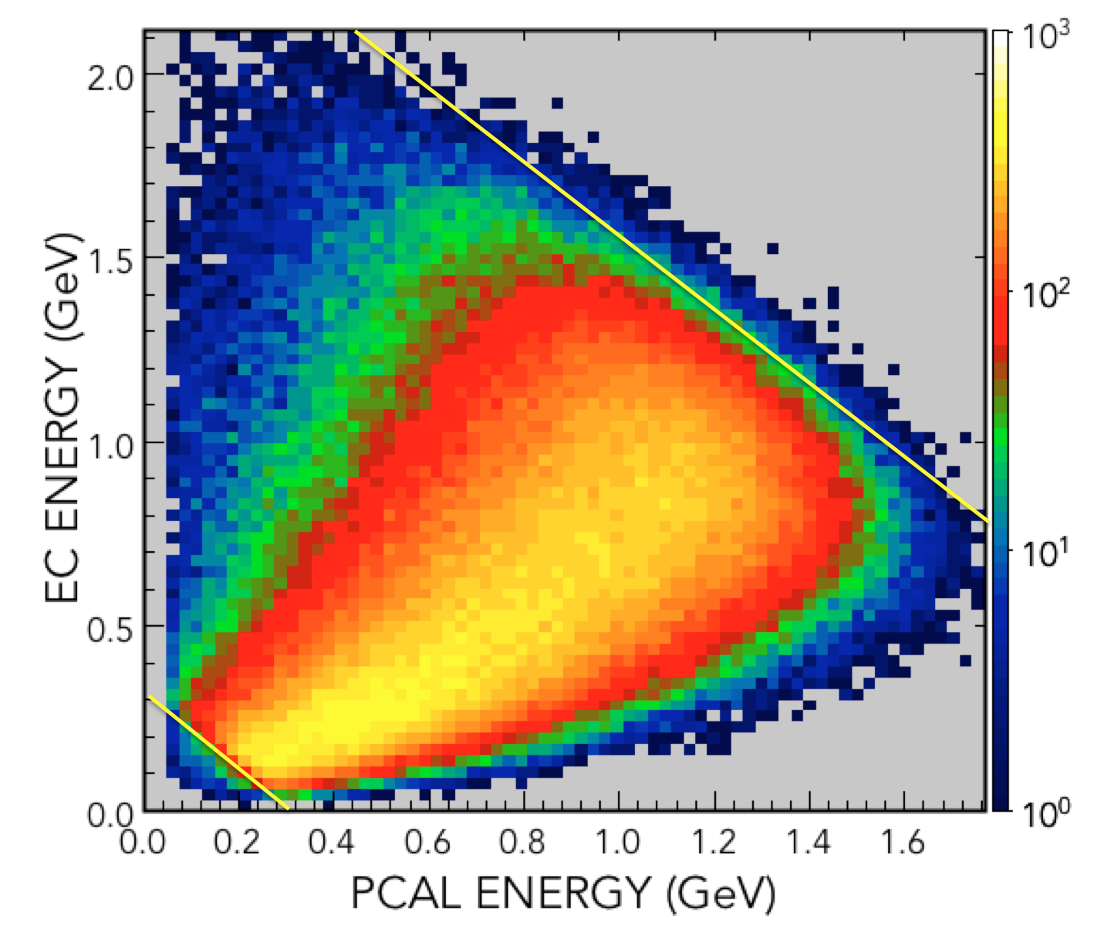
\includegraphics[width=0.8\columnwidth,keepaspectratio]{img/S10_1_000.png}
\caption[]{Reconstructed shower energy in the PCAL and EC modules in response to electrons with a momentum range of 1-10 GeV/c and a polar scattering angle range of 6-34 degrees.  The energy is not corrected for sampling fraction. Diagonal lines show the limits for the total reconstructed energy PCAL+EC.}
\label{fig:S10_1_000}
\end{figure}

\subsection{Electron Response}
The response of the PCAL and EC components of a single FEC module to high energy electrons is shown in Fig.~\ref{fig:S10_1_000}.  The beam energy was 10.6 GeV and outbending scattered electrons were selected by the Event Builder (EB) service by matching a negative charge forward track to FEC clusters in PCAL, ECIN and ECOU and requiring an activated High Threshold Cerenkov Counter (HTCC) mirror segment that matches the same track.  The plot clearly shows the correlations between energy reconstructed in the forward and rear sections of the FEC, while the logarithmic $z$-scale emphasizes the range of fluctuations. The diagonal lines are the total reconstructed  energy with the location of the total energy trigger threshold shown at PCAL+EC = 300 MeV and the other line showing the maximum deposited energy consistent with the scattering angle cutoff at $\theta_{elec}=6^o$. Contributions from pions that exceed the 4.7 GeV threshold cutoff of the HTCC were rejected in the hardware trigger using a PCAL energy threshold of 60 MeV.

The sampling fraction (SF) for electromagnetic showers is defined as the ratio of the total sampled energy (PCAL+EC) to the incident particle energy.  GEMC simulations of electrons impacting the central portion of the FEC show a SF dependence on measured energy ranging from 0.22 to 0.255 over the expected range of electron momentum.  The measured sampling fraction for electrons in the momentum range 1-10 GeV/c is shown in Fig.~\ref{fig:S10_1_0} and follows the expected trend, with some few percent systematic deviations due possibly to residual calibration errors.

\begin{figure}[t]
\centering
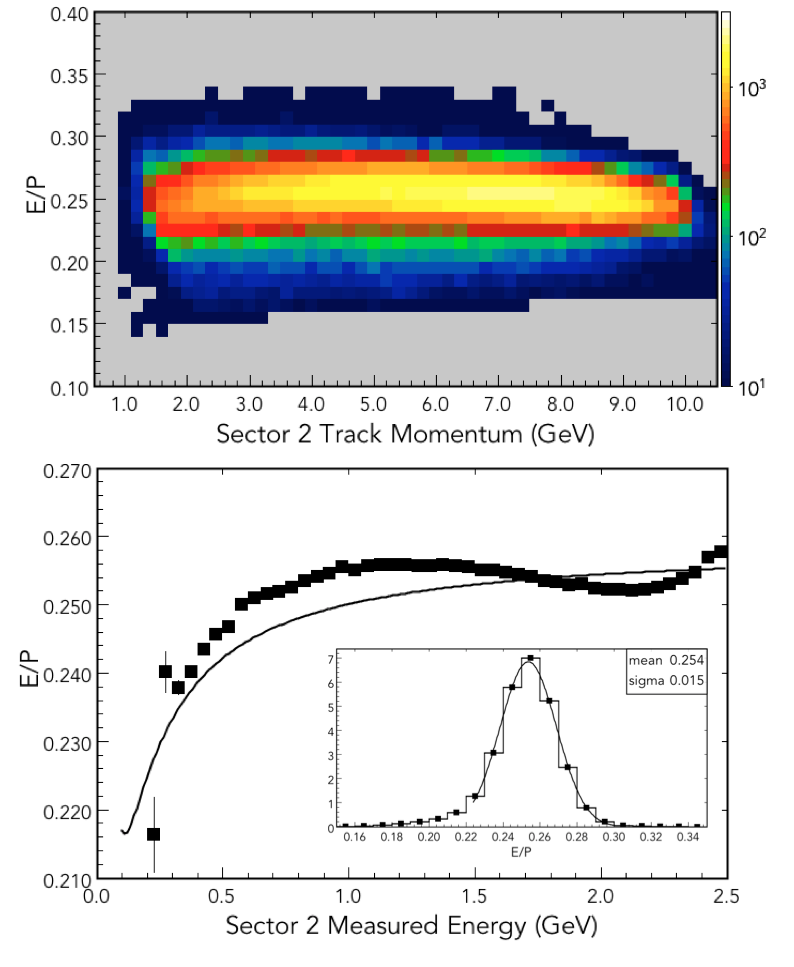
\includegraphics[width=1.0\columnwidth,keepaspectratio]{img/S10_1_0.png}
\caption[]{Top: Distribution of the ratio $E/P$ of the total reconstructed FEC energy to the momentum of outbending forward tracks linked to clusters in PCAL, ECIN and ECOU that were identified as electrons by the Event Builder service.  BOTTOM: $E/P$ versus FEC measured energy compared to GEMC prediction.  The inset shows a Gaussian fit to the overall $E/P$ distribution.}
\label{fig:S10_1_0}
\end{figure}

The variance of the sampling fraction can be expanded as a function of energy with the usual parameterization of contributions \cite{ps1981}:
\begin{equation}
\biggl[\frac{\sigma(E)}{E}\biggr]^2 = \frac{\sigma^2_0}{E^2} + \frac{\sigma^2_1}{E} +\sigma^2_2 + \sigma^2_3 E 
\label{eq:sferror}
\end{equation}

\begin{itemize}
\item $\sigma_0$ - Pedestal noise, cross-talk;
\item $\sigma_1$ - Poisson statistics (sampling, PMT);
\item $\sigma_2$ - Calibration errors (PMT gains);
\item $\sigma_3$ - Shower leakage fluctuations.
\end{itemize}

Typically $\sigma_0$ is ignored, although for MIP-based calibration analysis the contribution may be non-negligible.  To minimize this contribution all CLAS12 PMT data are taken with fADC pedestals measured and subtracted event-by-event.  Shower leakage contributions to $\sigma_3$ are most important for inbending electrons impacting the FEC at the forward-most angles, where there is incomplete overlap of PCAL and EC and vanishing acceptance.  

Estimates of the contributions from $\sigma_1$ and $\sigma_2$ were performed using fits to the expected linear dependence of the total relative variance on the inverse of the electron energy as shown in Fig.~\ref{fig:S10_1_1}.  The summary of these fits shows an average energy resolution of $\sigma_1 = 0.09$~GeV$^{1/2}$ which is consistent with expectations from GEMC.   The fit results for $\sigma_2$ of around $4\%$ is typical of the present instabilities of PMT gain matching.
 
\begin{figure}[t]
\centering
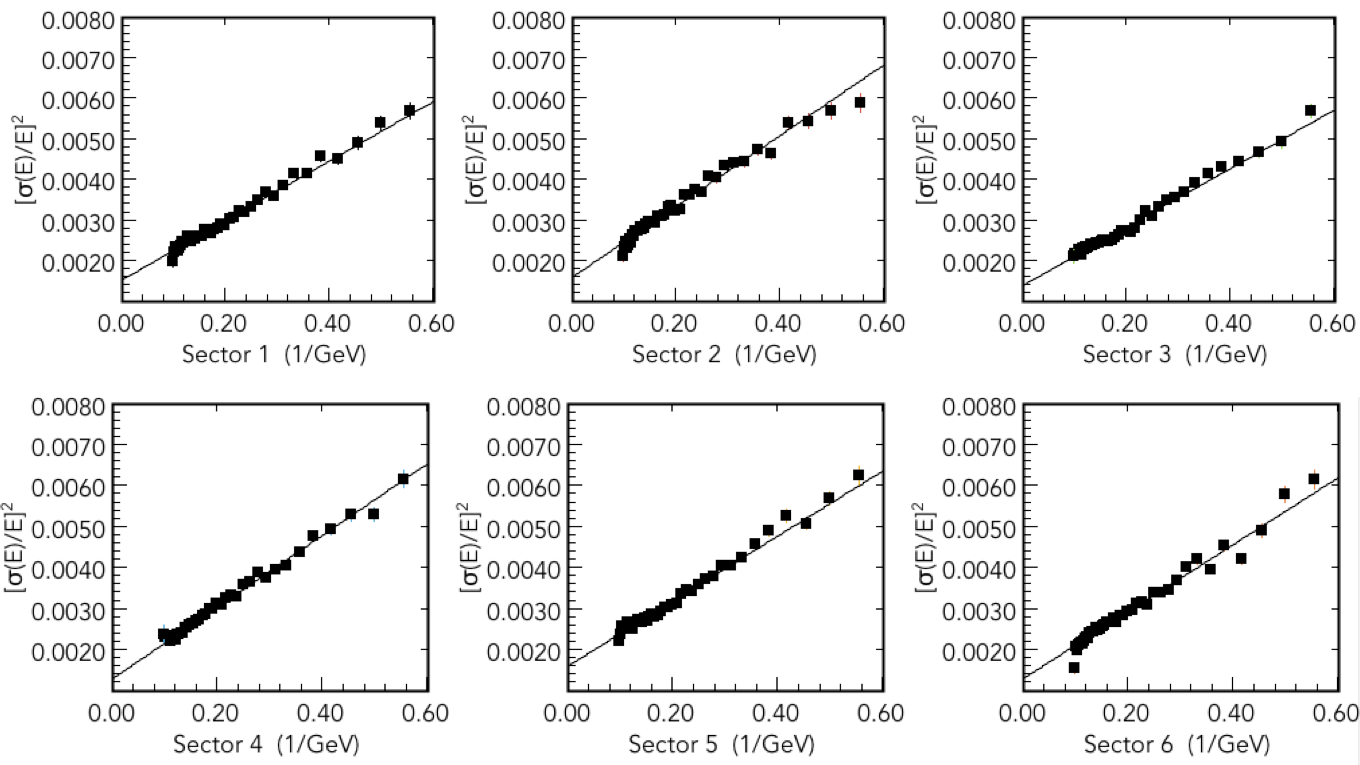
\includegraphics[width=1.0\columnwidth,keepaspectratio]{img/S10_1_1.png}
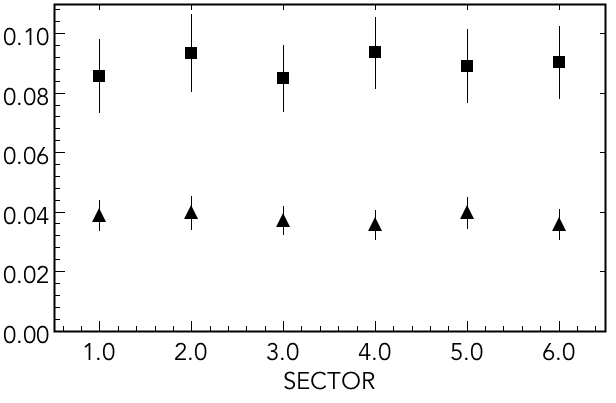
\includegraphics[width=0.5\columnwidth,keepaspectratio]{img/S10_1_2.png}
\caption[]{Relative variance of the measured sampling fraction plotted versus the inverse electron energy.  The linear fits used to obtain the resolution and calibration variance terms in Eq. 7 are summarized at the bottom, where $\sigma_1 (\blacksquare)$ and $\sigma_2 (\blacktriangle)$ are plotted versus sector.}
\label{fig:S10_1_1}
\end{figure}

\begin{figure}[t]
\centering
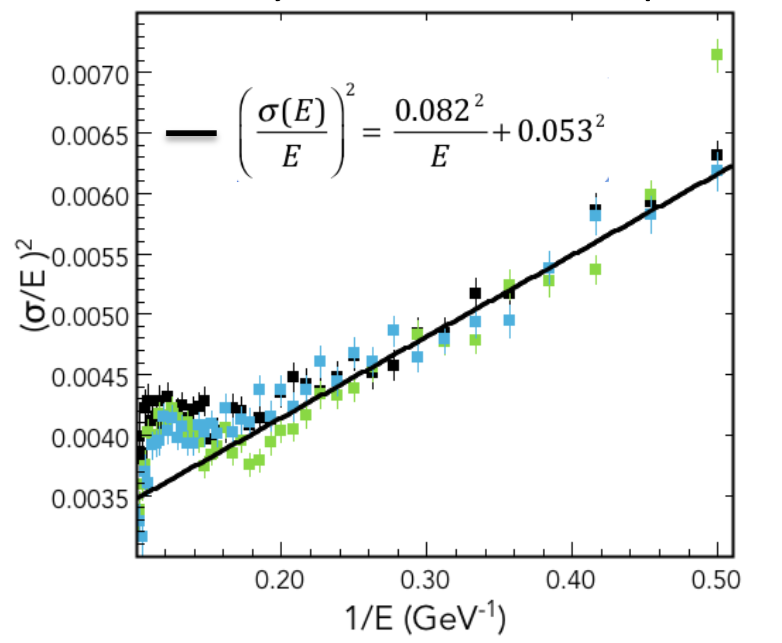
\includegraphics[width=1.0\columnwidth,keepaspectratio]{img/S10_1_3.png}
\caption[]{Top: Histograms show the distribution of residuals in Sector 3 between the projected hit position of forward tracks for electrons and the reconstructed PCAL cluster position for the radial (left) and transverse (right) coordinates. Bottom: Sector dependence of radial (black) and transverse (red) residuals for PCAL (left) and ECIN (right).  The error bars show the sigma of Gaussian fits to the residual distributions.}
\label{fig:S10_1_3}
\end{figure}

\subsection{Position Resolution}
The scintillator alignment and position resolution were estimated from comparison of the reconstructed position of shower clusters with the extrapolation of the forward tracking trajectory state vector of electron tracks from the target to the tracking planes of the PCAL and ECIN.  
Fig.~\ref{fig:S10_1_3} summarizes the electron track-cluster matching residuals in the tilted local sector frame.   Systematic offsets for the PCAL of $\approx 1$~cm and $\approx 0.5$ cm are seen in the radial (perpendicular to the U strips) and transverse (along the direction of the U strips) directions respectively.  These results are consistent with the present uncertainties in the scintillator location. The ECIN residuals have not changed from the CLAS era, although the fitted sigmas of the residual distributions are smaller, possibly due to the improved angular resolution of the CLAS12 forward tracking and smaller multiple scattering at 10 GeV.  The PCAL residual fits imply an angular resolution of $\approx 1.2$~mrad for showers in the Forward Detector.  The measured offsets, together with survey data, will be used to further optimize the track matching cuts used for electron ID and background rejection. 

\begin{figure}[t]
\centering
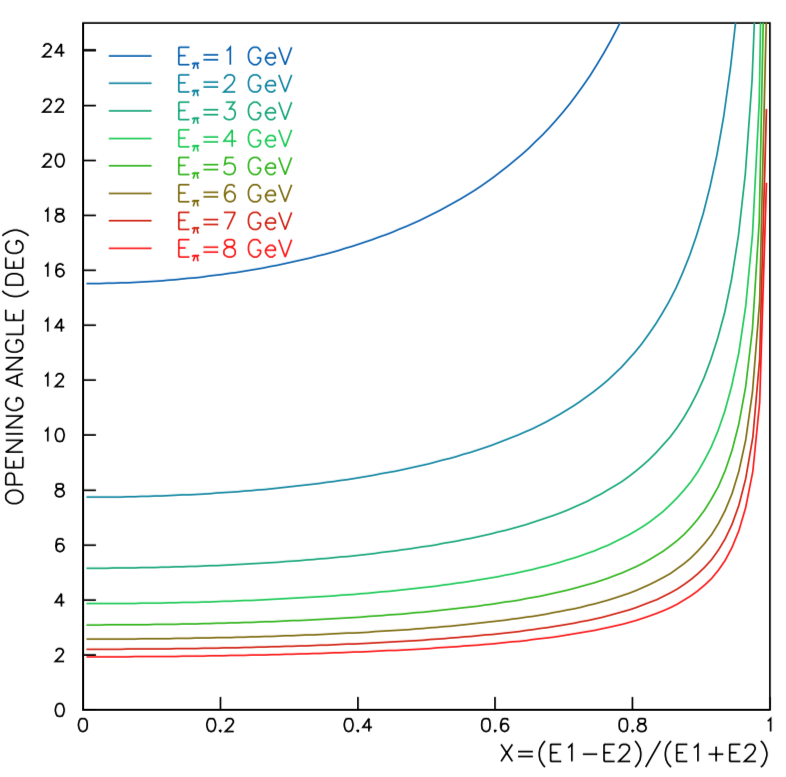
\includegraphics[width=0.7\columnwidth,keepaspectratio]{img/opa.png}
\caption[]{Opening angle of the $\pi^0 \rightarrow \gamma \gamma$ decay versus the energy asymmetry $X$ of the two photons, shown for the range of $\pi^0$ energies measured in CLAS12. }
\label{fig:opa}
\end{figure}

\subsection{Reconstruction of $\pi^0\rightarrow \gamma \gamma$ Decays}

Detection of the neutral pi meson requires reconstruction of the invariant mass of the $\pi^0 \rightarrow \gamma \gamma$ decay, using:
\begin{equation}
m^2 = 2 E_1 E_2 (1-\cos \theta_{12}),
\label{eq:ivm}
\end{equation}
 where $E_1$ and $E_2$ are the energies of the two photon showers in the FEC and $\theta_{12}$ is their opening angle with respect to the target vertex.  The meson energy can be determined from these same measurements in terms of the photon energy asymmetry $X$:
\begin{equation}
E^2_{\pi} = \frac{m^2_{\pi}}{(1-\cos \theta_{12})(1-X^2)}  \\
X=\frac{E_1-E_2}{E_1+E_2}
\label{eq:epi}
\end{equation}
The reaction kinematics following from Eqs.~\ref{eq:ivm} and \ref{eq:epi} are shown in Fig.~\ref{fig:opa}.  Clearly both the invariant mass and energy reconstruction are dominated by the FEC opening angle resolution and accuracy at the highest energies, while at lower energies both the energy and angle resolutions contribute.   Therefore this measurement can be used reveal and refine the systematics and consistency of the energy calibration, geometrical alignment and cluster reconstruction of the FEC.

\begin{figure}[h]
\centering
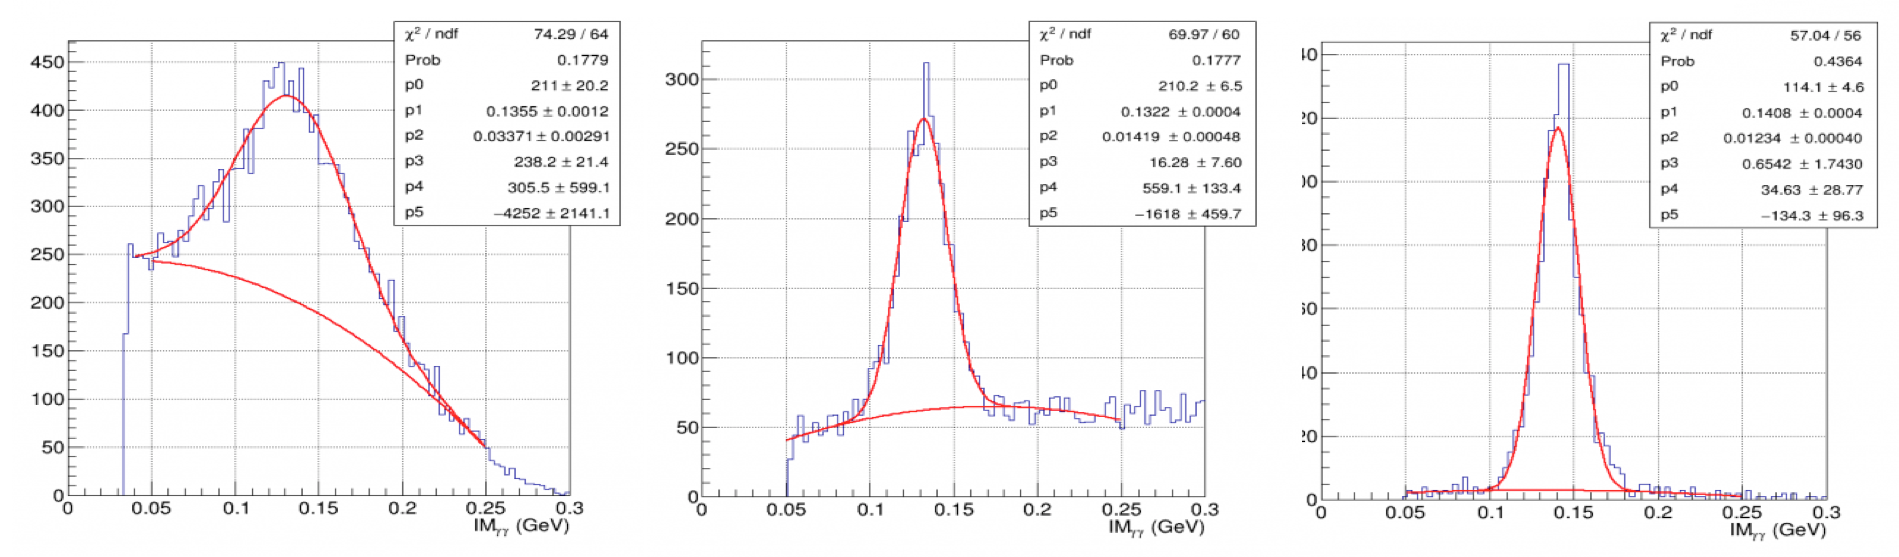
\includegraphics[width=1.0\columnwidth,keepaspectratio]{img/fx-pi0-fits.png}
\caption[]{Empirical fits to both the combinatorial background and the invariant mass peaks reconstructed from two photons detected in the same sector of the FEC.  These data represent symmetric $\pi^0 \rightarrow \gamma \gamma$ decays where both photons are within the energy bins indicated in the plot. Fits shown are for photon energies of $E_{\gamma}$ = 0.25, 0.75 and 2.75 GeV.}
\label{fig:fx-pi0-fits}
\end{figure}

An error analysis of Eq.~\ref{eq:ivm} leads to the following expression for the invariant mass resolution expressed in terms of the uncertainties of the measured quantities:
\begin{equation}
\sigma_m  = \frac{m_{\pi}}{2}\left[\left(\frac{\sigma(E_1)}{E_1}\right)^2 + \left(\frac{\sigma(E_2)}{E_2}\right)^2 + \sigma^2_{\theta_{12}}\frac{\sin^2 \theta_{12}}{(1-\cos \theta_{12})^2}\right]^{1/2}
\label{eq:sigmam1}
\end{equation}
For symmetric decays, where $E_1 \approx E_2$ or $X \rightarrow 0$, and using Eq.~\ref{eq:epi} and the dominant contributions to the photon energy resolution from Eq.~\ref{eq:sferror}, the invariant mass resolution $\sigma_m$ reduces to a dependence solely on the pion energy $E_{\pi}$:

\begin{equation}
\sigma_m = \frac{m_{\pi}}{2}\left[\frac{4 \sigma^2_1}{E_{\pi}} + 2 \sigma^2_2 + \sigma^2_{\theta_{12}}\left(\frac{4 E^2_{\pi}}{m^2_{\pi}}-1\right)^2\right]^{1/2}.
\label{eq:sigma2}
\end{equation}

Using Eq.~\ref{eq:sigma2} it is possible to identify the contributions to $\sigma_m$ due to energy resolution $\sigma_1$, calibration error $\sigma_2$, and opening angle resolution $\sigma_{\theta_{12}}$ by measuring the invariant mass as a function of pion energy.  This study was performed using a single 10.6 GeV run to accumulate a high statistics sample of symmetric $\pi^{0}$ decays.  Gaussian fits similar to those shown in Fig.~\ref{fig:fx-pi0-fits} were used to extract the mean and sigma of the invariant mass peak over a photon energy range of 0.2-4.0 GeV, corresponding to a pion energy range of 0.5-8.0 GeV.  Results from the fits are shown in Fig.~\ref{fig:fx-study-summary}, where a sector-based analysis (open symbols) and a global analysis summed over sectors (solid symbols) are plotted.  

The analysis of symmetric decays, which are kinematically over-constrained, also permits an estimate for the photon energy correction~\cite{2006015}, under the assumption that unphysical values of the invariant mass arise solely from this dependence.  The GEMC prediction of the photon sampling fraction for the FEC is shown by the solid line in Fig.~\ref{fig:fx-study-summary-2}.   The calculated energy dependence and absolute magnitude depend largely on the lead-scintillator design and details of the inert material between the PCAL and EC and pre-radiation in the materials in front of the FEC.  The fitted photon energy correction from the symmetric decay analysis is seen to follow the GEMC parameterization, with some systematic deviations that are being studied.  Our current physics analysis uses the GEMC result.


\begin{figure}[h]
\centering
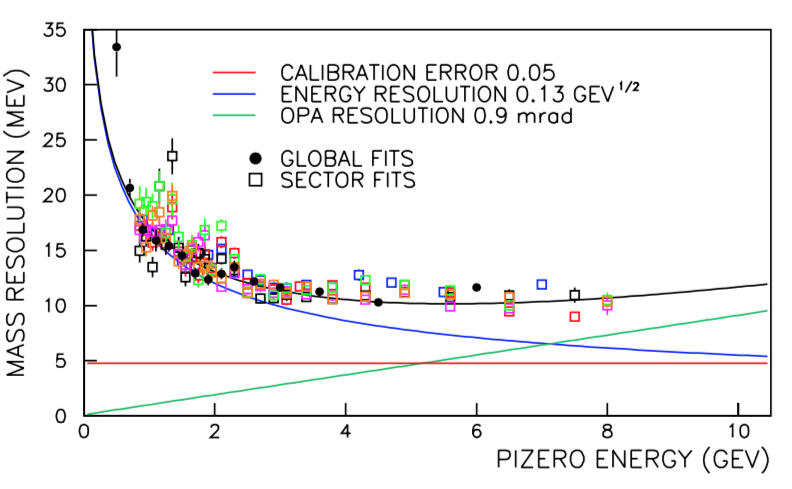
\includegraphics[width=1.0\columnwidth,keepaspectratio]{img/fx-study-summary.png}
\caption[]{Summary of fits to invariant mass peaks from $\pi^0 \rightarrow \gamma \gamma$ symmetric decays showing the mass resolution $\sigma_m$ versus $\pi^0$ energy.  A model of the mass resolution using Eq.~\ref{eq:sigma2} was fitted to the energy dependence of $\sigma_m$ to extract estimates of the photon energy and opening angle resolution, as well as the overall calibration uncertainty.}
\label{fig:fx-study-summary}
\end{figure}

\begin{figure}[h]
\centering
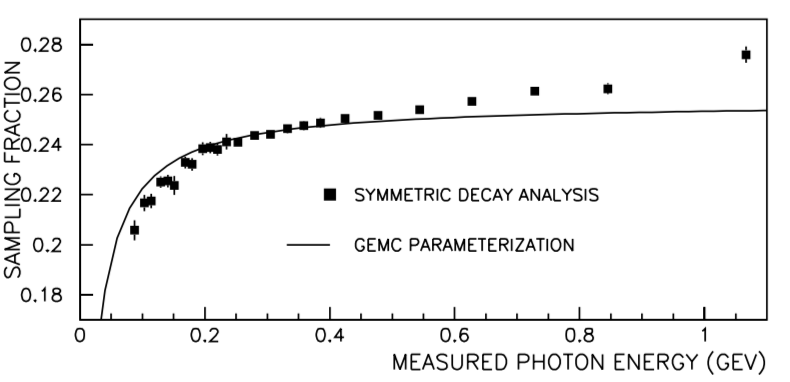
\includegraphics[width=1.0\columnwidth,keepaspectratio]{img/fx-study-summary-2.png}
\caption[]{Summary of fits to invariant mass peaks from $\pi^0 \rightarrow \gamma \gamma$ symmetric decays showing the fitted energy corrections to the measured photon energy.  The solid line shows the GEMC calculated photon sampling fraction.}
\label{fig:fx-study-summary-2}
\end{figure}

\subsection{Neutron Detection}
Clusters in the FEC not associated with any reconstructed forward track are designated neutrals by the Event Builder service.  Association of neutral PCAL clusters with ECIN and ECOU clusters are based on proximity to straight line trajectories from the scattering target centerline to the PCAL cluster.  Photons and neutrons are distinguished on the basis of the timing response, with neutrons defined as having velocity $\beta < 0.9$.  Experiments that require the exclusive measurement of neutrons in the FEC therefore require both good timing resolution and sufficient detection efficiency. 

\begin{figure}[h]
\centering
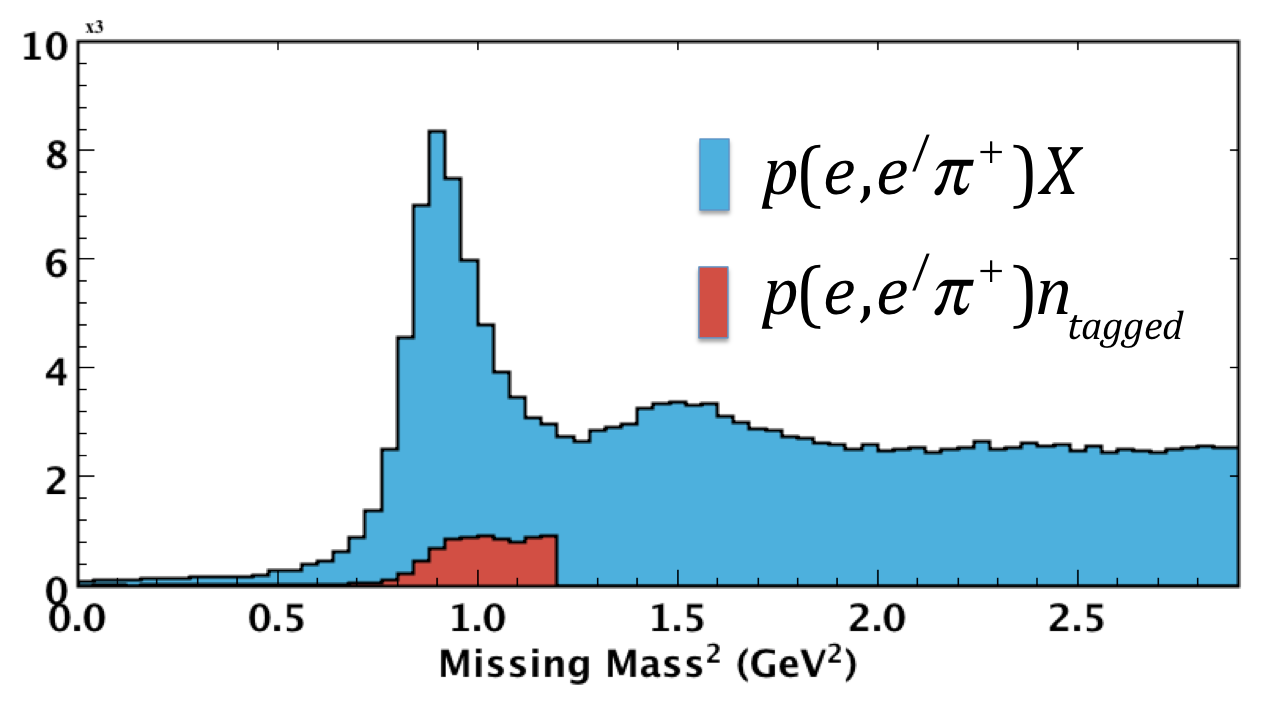
\includegraphics[width=1.0\columnwidth,keepaspectratio]{img/S10_4_0.png}
\caption[]{Missing mass $M_X$ distribution from detection of a $e^-~\pi^+$ final state using a proton target.  The beam energy was 7.6 GeV.  Single neutrons are identified with the cut $M_X < 1.2$~GeV and the fraction of tagged neutrons entering the FEC fiducial area are indicated in red. }
\label{fig:S10_4_0}
\end{figure}

\begin{figure}[h]
\centering
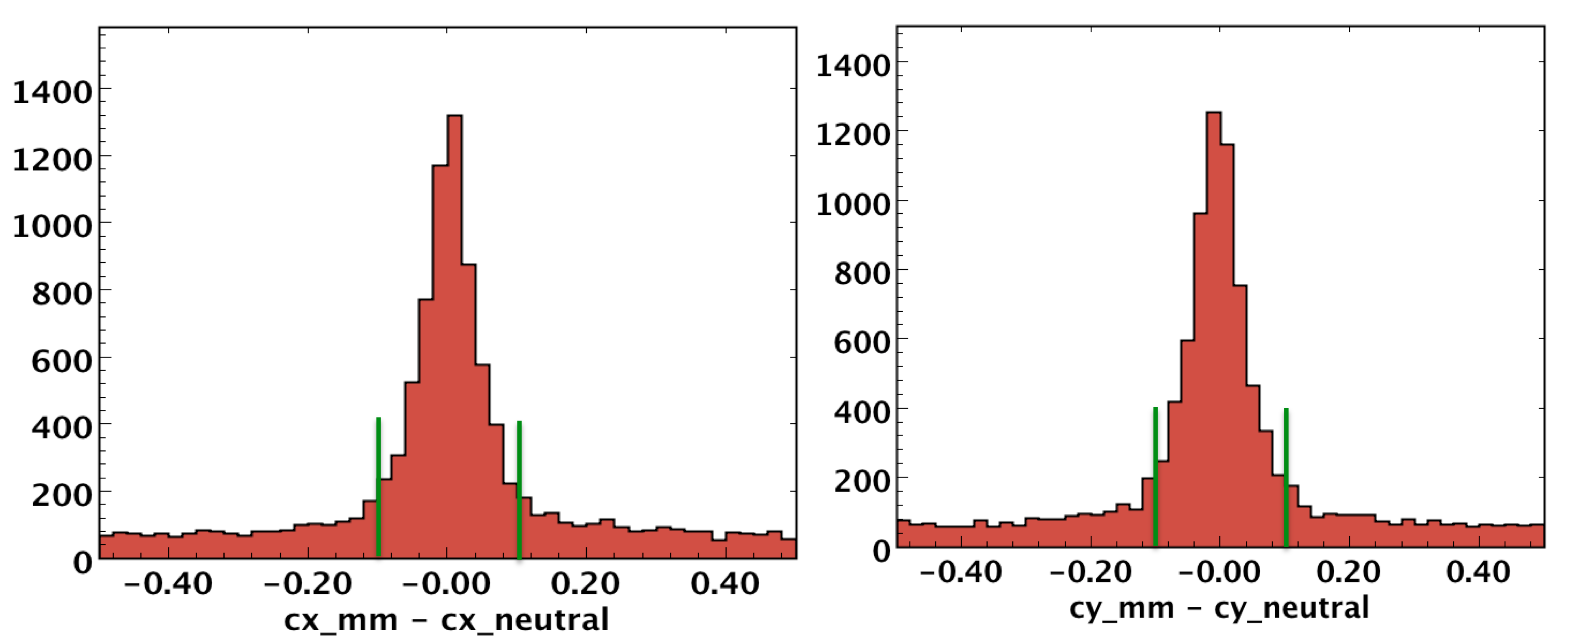
\includegraphics[width=1.0\columnwidth,keepaspectratio]{img/S10_4_1.png}
\caption[]{Differences in direction cosines between the missing momentum of the tagged neutron and the detected neutral cluster in the FEC.  The vertical lines show the cuts used to minimize the background from uncorrelated photons.}
\label{fig:S10_4_1}
\end{figure}

\begin{figure}[h]
\centering
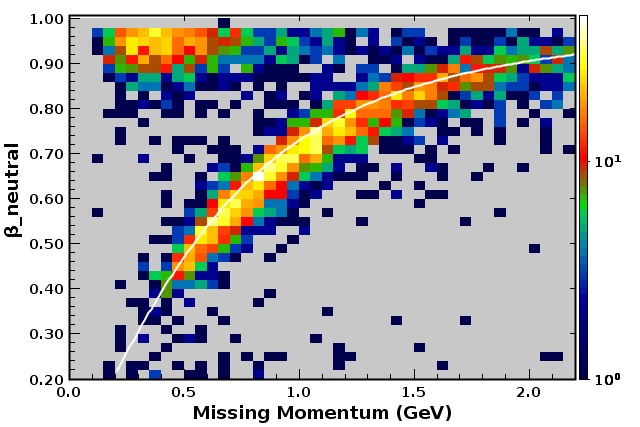
\includegraphics[width=1.0\columnwidth,keepaspectratio]{img/S10_4_2.png}
\caption[]{Correlation between the measured velocity $\beta$ of neutral clusters in the FEC and the missing momentum of the tagged neutron, subject to the $\Delta cx,\Delta cy$ cuts shown in Fig.~\ref{fig:S10_4_1}.  The black line shows the expected correlation for neutrons.}
\label{fig:S10_4_2}
\end{figure}

Neutron detection in the FEC was studied using the $p\,(\,e,e'\,\pi^+\,)\,n$ reaction to provide a source of tagged neutrons (Fig.~\ref{fig:S10_4_0}.) Data were taken with a 7.6 GeV beam energy.  Events with missing momentum pointing into the fiducial region of the FEC were selected.  Candidate neutron hits were identified by requiring the direction of the missing momentum to coincide with the direction of a measured neutral cluster within the expected angular resolution, assuming the target center as origin.  Typical cuts used for these kinematic residuals are shown in (Fig.~\ref{fig:S10_4_1}) for the direction cosines $cx$ and $cy$ of the neutron momentum vector with respect to the beamline.  Events that satisfy the angle cuts are plotted in Fig.~\ref{fig:S10_4_2}.  The data show a clear correlation with the tagged neutron momentum and agrees with the expected correlation (black line) for a particle with the neutron mass.  Some photon background is also visible, most likely from beam related accidentals. The resulting mass squared $M^2$ distribution calculated from the measured $\beta_{neutral}$ and missing momentum is shown in Fig.~\ref{fig:S10_4_3} (left), where the photon and neutron peaks are clearly separated.  Neutrons were selected using the cut $M^2 > 0.45$~GeV$^2$ and identical acceptance fiducial cuts were placed on both tagged and measured neutrons.  The ratio of the detected and tagged neutrons is shown in Fig.~\ref{fig:S10_4_3} (right).  The efficiency follows the trend expected from GEMC/GEANT4 simulations but the absolute magnitude is about a factor of two low.  At the present level of CLAS12 event reconstruction this is acceptable, as further improvements in the missing mass resolution,  rejection of photon accidentals in the FEC and compensation for low energy deposition losses in the aging EC should improve the accuracy of both the numerator and denominator of the efficiency ratio. 

\begin{figure}[h]
\centering
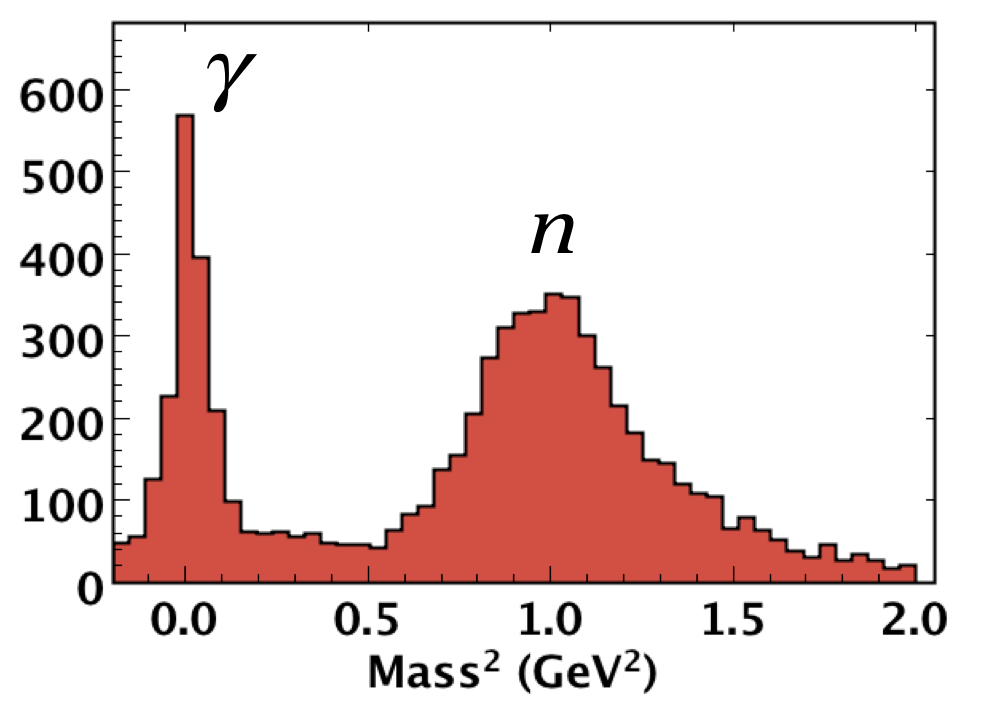
\includegraphics[width=1.0\columnwidth,keepaspectratio]{img/S10_4_3.png}
\caption[]{Left: Mass distribution of neutrals detected in the PCAL and EC calculated from the measured $\beta$ and missing momentum of tagged spectator neutrals.  Both photon and neutron peaks are visible. Right: Efficiency for detection of tagged neutrons.  A cut of $M^2>0.45$ GeV$^2$ was used to reject photons.  Identical fiducial acceptance cuts were applied to both tagged and measured neutrons.}
\label{fig:S10_4_3}
\end{figure}



